\ProvidesFile{ch-light-curve-inversion.tex}[Light Curve Shape Inversion]
\graphicspath{{/Users/liamrobinson/Documents/msthesis/static_images/aas_2022_figs}}
\section{Light Curve Shape Inversion}

\subsection{Direct Convex Shape Inversion}

Traditionally, direct light curve inversion involves two distinct optimization problems: a linear least squares problem to fit an EGI to the measured light curve, and a second optimization to produce accurate vertex positions and face adjacency information \cite{fan2020thesis}. The first problem is data-driven and linear, using the observations to estimate a plausible EGI. The second problem is highly nonlinear but convex and requires significant tuning for robust convergence \cite{fan2019}.

\subsubsection{The Extended Gaussian Image} \label{sec:egi_definition}

The discrete EGI $\vec{E} \in \mathbb{R}^{m \times 3}$ is composed of $m$ unit vectors $\hat{n}$ each scaled a nonnegative scalar $a \in \mathbb{R}$, where $a_i \geq 0 \forall i$ \cite{little1983}.

\begin{equation}
  \vec{E}_i = a_i \hat{n}_i
\end{equation}

In the context of shape inversion, the $m$ vectors $\hat{n}$ should be a relatively uniform tessellation of the unit sphere. A convex polytope can be uniquely represented by an EGI of facet normal vectors scaled by each facet's area. The set of normal vectors in an EGI is denoted $\mathcal{N}$ with the set of areas denoted $\mathcal{A}$. The vector of facet areas is denoted $\vec{a} \in \mathbb{R}^{m \times 1}$. The norm of the EGI is notated $\| \vec{E} \| = \vec{a}$ with the `size' of the EGI $\|\vec{E}\| = m$.

The solution to the Minkowski problem proves the existence and uniqueness of a convex polytope for any EGI satisfying the closure condition \cite{minkowski1909}:

\begin{equation} \label{eq:egi_closure}
  \sum_{i=1}^m a_i \hat{n}_i = [0, 0, 0].
\end{equation}

Equivalently, an EGI uniquely represents a closed, convex polyhedron --- a polytope --- with no open boundaries, up to a translation. While a given EGI uniquely represents a polytope, that same EGI could also be interpreted to be an infinite number of nonconvex and open geometries. An example of this extended family is depicted in Figure \ref{fig:egi_family}.

\begin{figure}[!htb]
  \centering
  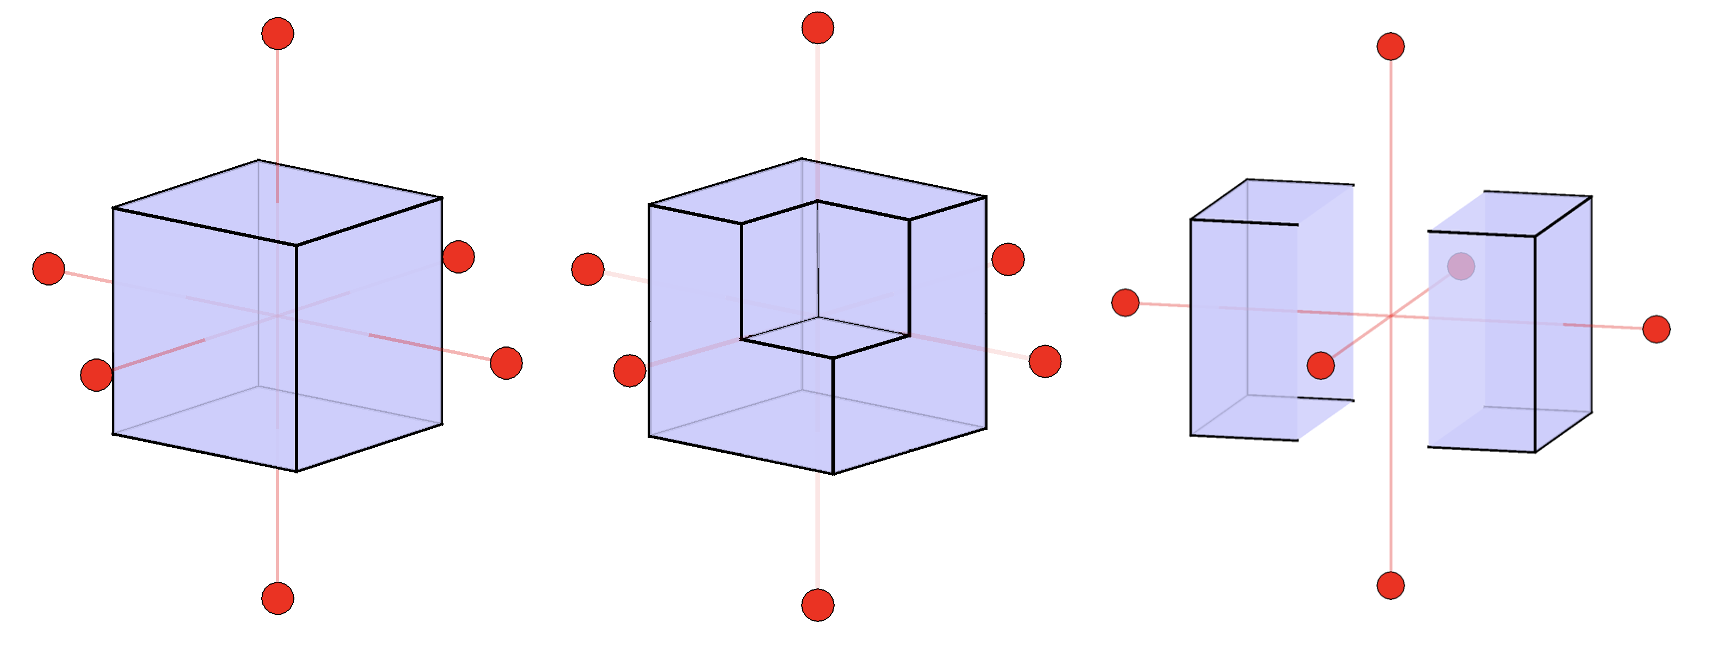
\includegraphics[width=\figmed]{convex_non_open_egis.png}
  \caption{Simplified convex, nonconvex, and open EGI nonuniqueness. Larger circles indicate greater relative areas assigned to a given normal vector.}
  \label{fig:egi_family}
\end{figure}

\subsubsection{EGI Optimization}

The EGI fulfills two important criteria for the shape inversion problem: it can be estimated directly from the light curve, attitude profile, and material properties, and uniquely represents a convex object \cite{kaasalainen2001}. Further, the EGI can be transformed into a unique convex object and vice versa through the dual transform and Minkowski problem \cite{little1985, minkowski1909}. 

Given a light curve, direct shape inversion schemes sample $m$ candidate normal vectors $\hat{n}$ on the unit sphere to fit an EGI to the observed light curve $\vec{L}_\textrm{ref} \in \mathbb{R}^{n \times 1}$ \cite{friedman2020, fan2020thesis}. This is accomplished by solving an optimization problem to distribute the area vector $\vec{a}$ across the sampled normals to minimize the residual between the observed and modeled light curves. In practice, this is a constrained nonnegative least squares (NNLS) problem and can be solved efficiently for large numbers of normal vectors and light curve data points:

\begin{equation} \label{eq:area_opt_convex}
  \min_{a}{\|\vec{L}_{\textrm{ref}} - G \vec{a}\|_2} \:\:\: \textrm{ subject to } \vec{a}_i \geq 0.
\end{equation}

NNLS problems are efficiently solved via Lawson and Hanson's original algorithm \cite{lawson1976}, or the more recent Fast NNLS (FNNLS) algorithm due to Bro and De Jong \cite{bro1996}. It is important to note that the area estimated with Eq \ref{eq:area_opt_convex} is the \textit{albedo-area} due to the reflectivity coefficients in Eq \ref{eq:lc_func_normalized} or \ref{eq:lc_normalized_engine}. If the value of $C_d$ and $C_s$ are uniform with a known ratio $C_d / C_s$, the recovered geometry will be scaled without impacting the face adjacency or relative feature sizes.

The convex reflection matrix $G \in \mathbb{R}^{n \times m}$ with $ij$th entries $G_{ij}$ defined at time $i$ for each facet $j$ is defined as the normalized received facet irradiance per unit facet area:

\begin{align*} \label{ref_cond_matrix}
  G_{ij} &= \frac{I_{ij}}{I_0 a_j} \\
  &= f_r\left(L \rightarrow O \right) \left(L_j \cdot N_i\right) \left(O_j \cdot N_i\right).
\end{align*}

This relationship between the received normalized irradiance and the areas of the object faces reveals a more compact form of Eq \ref{eq:lc_func_normalized} for convex objects for any BRDF:

\begin{equation} \label{convex_lc_with_g}
  \hat{I}_{convex} = G \vec{a}.
\end{equation}

The optimization in Eq. \ref{eq:area_opt_convex} produces a coarse approximation of the true EGI as $m$ is finite. Increasing $m$ necessarily improves the quality and sparsity of the estimated EGI, but at the cost of computational resources. The estimation was performed using a synthetic light curve input from $n=500$ Sun and observer vectors uniformly sampled on the sphere in the body frame, producing a full rank $G$ matrix. $m = 500$ candidate normal vectors were sampled using a spherical Fibbonaci mapping described by Keinert et al. in \cite{keinert2015}. Results are visualized for an icosahedron in the body frame in Figure \ref{fig:initial_egi_sampling}. Reconstructing the object at this stage is difficult due to the quantity of faces present in the estimated EGI. 

\graphicspath{{/Users/liamrobinson/Documents/PyLightCurves/docs/build/html/_images}}
\begin{figure}[!htb]
  \centering
  \includegraphics[width=\figmed]{sphx_glr_egi_figs_aas22_002.png}
  \caption{Initial EGI optimization example for a cube, using 500 candidate normal vectors, the Phong BRDF with $C_d=0.5$, $C_s=0.5$, $n=10$. Relative face area denoted by higher sphere opacity, reference shape shown in grey.}
  \label{fig:initial_egi_sampling}
\end{figure}

\subsubsection{EGI Resampling}

A normal vector resampling step is presented in this work to promote a more accurate and sparse EGI. The normal vectors used in Fig \ref{fig:initial_egi_sampling} are generally correct, with each group clustering around a normal vector of the truth geometry. This clustering behavior occurs when none of the candidate normal vectors are sufficiently close to the truth. Resampling in a cone centered on each initial EGI normal vector provides more accurate candidates for EGI estimation. This process mimics a single optimization step with a much larger $m$, where the coarse EGI is used to exclude areas on the sphere with little or no normal area.

Uniformly sampling a cone of half-angle $\phi$ is accomplished by strategically sampling points on the unit sphere. 

\begin{equation} \label{cone_sample_n_pole}
  \hat{n}_{cone} = \begin{bmatrix}
    \sqrt{1-z^2}\cos{\theta} \\
    \sqrt{1-z^2}\sin{\theta} \\
    z \\
  \end{bmatrix}
\end{equation}

In Eq \ref{cone_sample_n_pole} two coordinates are chosen $z \in [\cos{\phi}, 1]$ and $\theta \in [0, 2\pi)$, yielding a point uniformly distributed on a cone of half-angle $\phi$ about the central axis $[0, 0, 1]^T$ \cite{cone_sampling_wolfram}. These points are then rotated using a direction cosine matrix to center the cone on an axis of interest. The axis of rotation for this transformation is the cross product of the original central axis $[0, 0, 1]^T$ with the final axis $\hat{n}_{cone}$ with the rotation angle $\theta$ being the angle between the same two vectors. The principal rotation parameter form of this transformation is given in Eq \ref{eq:cone_sampling_rv} which can be converted into the DCM using Eq \ref{eq:quat2dcm} and \ref{eq:prp2quat}.

\begin{align*} \label{eq:cone_sampling_rv} \numberthis
  \theta &= \cos^{-1}\left( \hat{n}_{cone,z} \right) \\
  \lambda &= \hat{n}_{cone} \times [0, 0, 1]^T
\end{align*}

The number of new candidates sampled per initial solution vector and the cone half-angle should be adjusted on a case-by-case basis depending on the compute power available and light curve data quality. Multiple iterative methods exist for solving nonnegatively constrained least squares (NNLS) problems. The classical NNLS algorithm was published by Lawson and Hanson and improved later by Bro and De Jong in their Fast NNLS (FNNLS) approach \cite{lawson1976, bro1996}.

Existing EGI optimization schemes like those of Fan \cite{fan2020thesis}, Friedman \cite{friedman2020}, and Cabrera \cite{cabrera2021} are limited by a single normal vector sampling step, leading to a lack of sparsity in the optimized EGI. High-density normal vector sampling in regions known to contain non-zero area leads to EGI solutions that are generally more sparse and cluster more tightly about true normal vectors. An example of this process is shown in Figure \ref{fig:resampled_egi}.

\begin{figure}[!htb]
  \centering
  \includegraphics[width=\figmed]{sphx_glr_egi_figs_aas22_003.png}
  \caption{Resampled EGI for the cube data using $\phi = \frac{\pi}{20}$, $100$ candidate vectors per resampled cone. Relative face area denoted by higher sphere opacity, reference shape shown in grey.}
  \label{fig:resampled_egi}
\end{figure}

\subsubsection{EGI Merging}

After resampling and reoptimizing with Eq. \ref{eq:area_opt_convex}, the reestimated EGI is merged by computing all groups $\mathcal{G}$ of EGI vectors within an angular offset $\alpha$:

\begin{equation}
  \mathcal{G}_k = \left\{ \vec{E}_i \in \vec{E} \:\| \cos^{-1}\left( \frac{\hat{E}_i \cdot \hat{E}_k}{\|\vec{E}_i \| \| \vec{E}_k \|}\right) < \alpha \right\}.
\end{equation}

In practice, the choice of $\alpha$ is dependent on the user's tolerance for discretization, as merging will approximate smooth geometry by discrete faces with normal vectors offset by $2\alpha$. Groups are merged by summing all group members, yielding a single EGI vector $\vec{E}_m$ without loss of closure. 

\begin{equation} \label{eq:fixing_egi}
  \vec{E}_m = \sum_{\vec{E} \in \mathcal{G}_k}{\vec{E}}
\end{equation}

Merging the resampled EGI shown in Figure \ref{fig:resampled_egi} produces a final sparse EGI fit for object reconstruction, shown in Figure \ref{fig:merged_egi}. 

\begin{figure}[!htb]
  \centering
  \includegraphics[width=\figmed]{sphx_glr_egi_figs_aas22_004.png}
  \caption{Merged EGI for the cube data using $\alpha = \frac{\pi}{10}$. Relative face area denoted by higher sphere opacity, reference shape shown in grey.}
  \label{fig:merged_egi}
\end{figure}
\graphicspath{{/Users/liamrobinson/Documents/msthesis/static_images/aas_2022_figs}}

\subsubsection{Geometry Recovery from the EGI}

At this stage, the resampled and merged EGI encodes a convex approximation of the underlying object with no guarantee of the closure of this EGI. The EGI closure constraint Eq \ref{eq:egi_closure} motivates a simple procedure to correct an invalid EGI by adding the mean closure error to each entry:

\begin{equation} \label{eq:egi_validation}
  \vec{E}_{\textrm{closed}} = \vec{E}_{\textrm{open}} - \sum_{i=1}^m a_i \hat{n}_i .
\end{equation}

The concept of a closure step is not a novel contribution. Fan's method solved an optimization problem to adjust the EGI towards closure \cite{fan2020thesis}. This process is inproved with a simpler analytical correction. In practice this process should be performed before each reconstruction to accelerate convergence. Failing to correct non-closed EGIs will cause convergence to a nonzero minimum in the reconstruction objective function as there is no corresponding convex object with the given EGI.

The unique convex object encoded by each closed EGI is reconstructed by solving for the polytope's set of vertices $\mathcal{V}$ and faces $\mathcal{F}$ encoding the adjacency relations between vertices. This is accomplished following the procedure introduced by Little through the dual transformation \cite{little1983}. The dual set $\mathcal{D}$ are vertices in $(A, B, C) \in \mathbb{R}^3$ that satisfy the following plane condition for a point $(x, y, z)$ on each face of the object:

\begin{equation} \label{eq:dual_abc_form}
  Ax + By + Cz + 1 = 0
\end{equation}

If $(x, y, z)$ are chosen to be the closest points in the object's planes to the origin, the dual set $\mathcal{D}$ can be expressed in terms of the EGI and a support vector $\vec{h} \in \mathbb{R}^{\|F\| \times 1}$, where the support vector is the vector of perpendicular distances of each face of the object to the origin. The dual is expressed in terms of the EGI and the supports as:

\begin{equation} \label{eq:dual_egi_form}
  \mathcal{D} = \frac{\vec{E}}{ \| \vec{E} \| \vec{h}}.
\end{equation}

The object's vertices $\vec{v}_{ref}$ are found by solving a linear system of equations for each face on the convex hull of dual set vertices. Triplets of vertices on the resulting faces are used to find a single real vertex by intersecting the three planes defining the dual set vertices.

\begin{equation} \label{eq:vertex_recovery}
  \begin{bmatrix}
    v_{ref,x} \\
    v_{ref,y} \\
    v_{ref,z} \\
  \end{bmatrix} = \begin{bmatrix}
    v_{i,x} & v_{j,x} & v_{k,x} \\
    v_{i,y} & v_{j,y} & v_{k,y} \\
    v_{i,z} & v_{j,z} & v_{k,z}
  \end{bmatrix}^{-1} \begin{bmatrix}
    1 \\ 1 \\ 1
  \end{bmatrix}
\end{equation}

Convex face adjacency information is found by triangulating the convex hull of all reference vertices. The accuracy of the recovered geometry is entirely dependent on the correctness of the support vector $\vec{h}$ used to produce the dual set. Finding the true support vector is the challenge of the final optimization in convex shape inversion.

\subsubsection{Support Vector Optimization}

This work adopts the same objective function proposed by Little for the support vector optimization as used by Fan \cite{little1983, fan2020thesis}. Little's objective function leverages work of Minkowski, who proved that any closed EGI is a unique representation of a convex object, up to a translation \cite{little1983}. In the literature, these convex shapes in $\mathbb{R}^3$ are known as polytopes. In particular, that unique polytope is merely a scaling and translation from the polytope with volume $1$ that minimizes $\vec{h} \cdot \| \vec{E} \|$ \cite{little1985}. This formulates the support vector optimization problem:

\begin{align*} \numberthis \label{eq:little_problem}
  & \min_{\vec{h}}\left\{ \vec{h} \cdot \| \vec{E} \| \right\} \\
  & \textrm{such that } \frac{1}{3}\left(\vec{h} \cdot \vec{a} \right) = 1
\end{align*} 

Notice that there is a difference between $ \| \vec{E} \| $, the areas of the faces on the desired polytope, and $\vec{a}$, the areas of the polytope recovered by constructing a convex object with the dual transform using Eqs \ref{eq:dual_egi_form} and \ref{eq:vertex_recovery}. This means that a convex object must be fully constructed at each step of the optimization to compute the objective function value. This optimization is highly nonlinear, as adjusting the support of one face may dramatically change the both the areas of surrounding faces as well as the volume of the resulting polytope. Due to the convexity of the problem, an initial guess of $\vec{h} = \mathbf{1}$ is sufficient.

Depending on the optimizer, additional function evaluations will be needed to evaluate support gradient as well as the Jacobian of the constraints. Many optimizers struggle with this optimization problem, either due to an inability to meet the constraint or instability that leads to unbounded supports. Little implemented a constrained gradient descent scheme from scratch, showing good results for reconstructing simple objects \cite{little1983}. Gardner solved an equivalent optimization problem using an unspecified solver in MATLAB \cite{gardner2003}. In this work, trust-region methods \cite{conn2000} were found to be robust at solving this optimization.

\subsection{Direct Nonconvex Shape Inversion}

\subsubsection{Nonconvex Feature Detection and Location}

Many human-made space objects are, as highlighted in Figure \ref{hst_bennu_shadows}, highly nonconvex. As a result, their shape inversion is plagued by the fact that the Minkowski problem-driven reconstruction methods of Eq \ref{little_problem} cannot recover nonconvex features. Instead of beginning from the ground up, the convex shape guess can be leveraged to detect and locate concavities.

Information about large, unilateral object concavities is obtained during EGI estimation in Eq. \ref{eq:area_opt_convex} by relaxing the EGI closure constraint. This unconstrained form is also generally functional for most convex objects and can be used without loss of detail in the final reconstruction as long as closure correction in Eq. \ref{eq:fixing_egi} is still employed.

The mean axis of prominent concave features is determined by measuring the divergence of the optimized EGI from a closed object with the magnitude of the closure error $\vec{e}_{EGI}$.

\begin{equation} \label{eq:closure_error}
  \vec{e}_{EGI} = -\sum_{i=1}^{m} a_i \hat{n}_i.
\end{equation}

The EGI closure error vector in Eq \ref{eq:closure_error} represents the missing area on each body axis that could be added to close the object. The addition of the minus sign transforms the vector from expressing the presence of excess area to the absence of missing area. The closure error will be negligible if there are no concavities present. The closure error may also be negligible if there is no self-shadowing is present over the sampled attitude profile, therefore the closure error merely quantifies the self-shadowing present in the measurements, not whether there may be self-shadowing in other orientations.

Under the strong assumption that the concavities present are major and unilateral, this EGI error vector points along the mean axis of the concavity. This is because self-shadowing in that region causes brightness measurements to be smaller than expected for the true area present, leading to an optimized EGI that attributes less area to that section of the object. As a result, summing the EGI entries produces a vector that points away from the concavity, requiring the negation seen in Eq \ref{eq:closure_error} to point towards it.

\subsubsection{Concavity Creation}

Given the direction of a supposed concavity in the body frame of the object, the next challenge is introducing that concavity. This work approximates unknown concave features as valleys with sharp floors, adopting the interior angle $\psi$ between the valley walls as the measure of the feature depth. An interior angle of $\psi=180^\circ$ implies no concavity, whereas $\psi \rightarrow 0^\circ$ will push the concavity through the object entirely.

The proposed process for creating an accurate concavity in the reconstructed convex guess proceeds in four major steps. The model is first subdivided to add more faces and vertices. Subdivided vertices are then classified by their proximity to the EGI error vector, indicating whether their positions should be updated. Boundary vertices are identified, and vertex positions are updated based on an internal angle. The light curve error of that nonconvex guess is computed, and the internal angle is iterated until a suitable minimum error case is identified.

\subsubsection{Model Subdivision}

Subdividing the initial convex object guess is essential for retaining object detail during concavity creation. A combination of linear subdivision, Loop subdivision, and remeshing algorithms are used to accomplish this. Linear subdivision is advantageous when object faces are equally sized and boundary edges must be maintained. Loop subdivision is preferable when there are numerous vertices so that subdivisions do not drastically diverge from the initial boundary surface. Loop subdivision softens sharp edges as it relies on B-splines to interpolate new vertex positions \cite{loop1987}. The specific type and resolution of subdivision used depends on the level of detail the user needs to maintain in the introduced concavity, although linear subdivision followed by Loop subdivision is a useful baseline. Varying combinations of subdivision are shown in Figure \ref{fig:subd_grid} to illustrate the available configurations.

\begin{figure}[!htb]
  \centering
  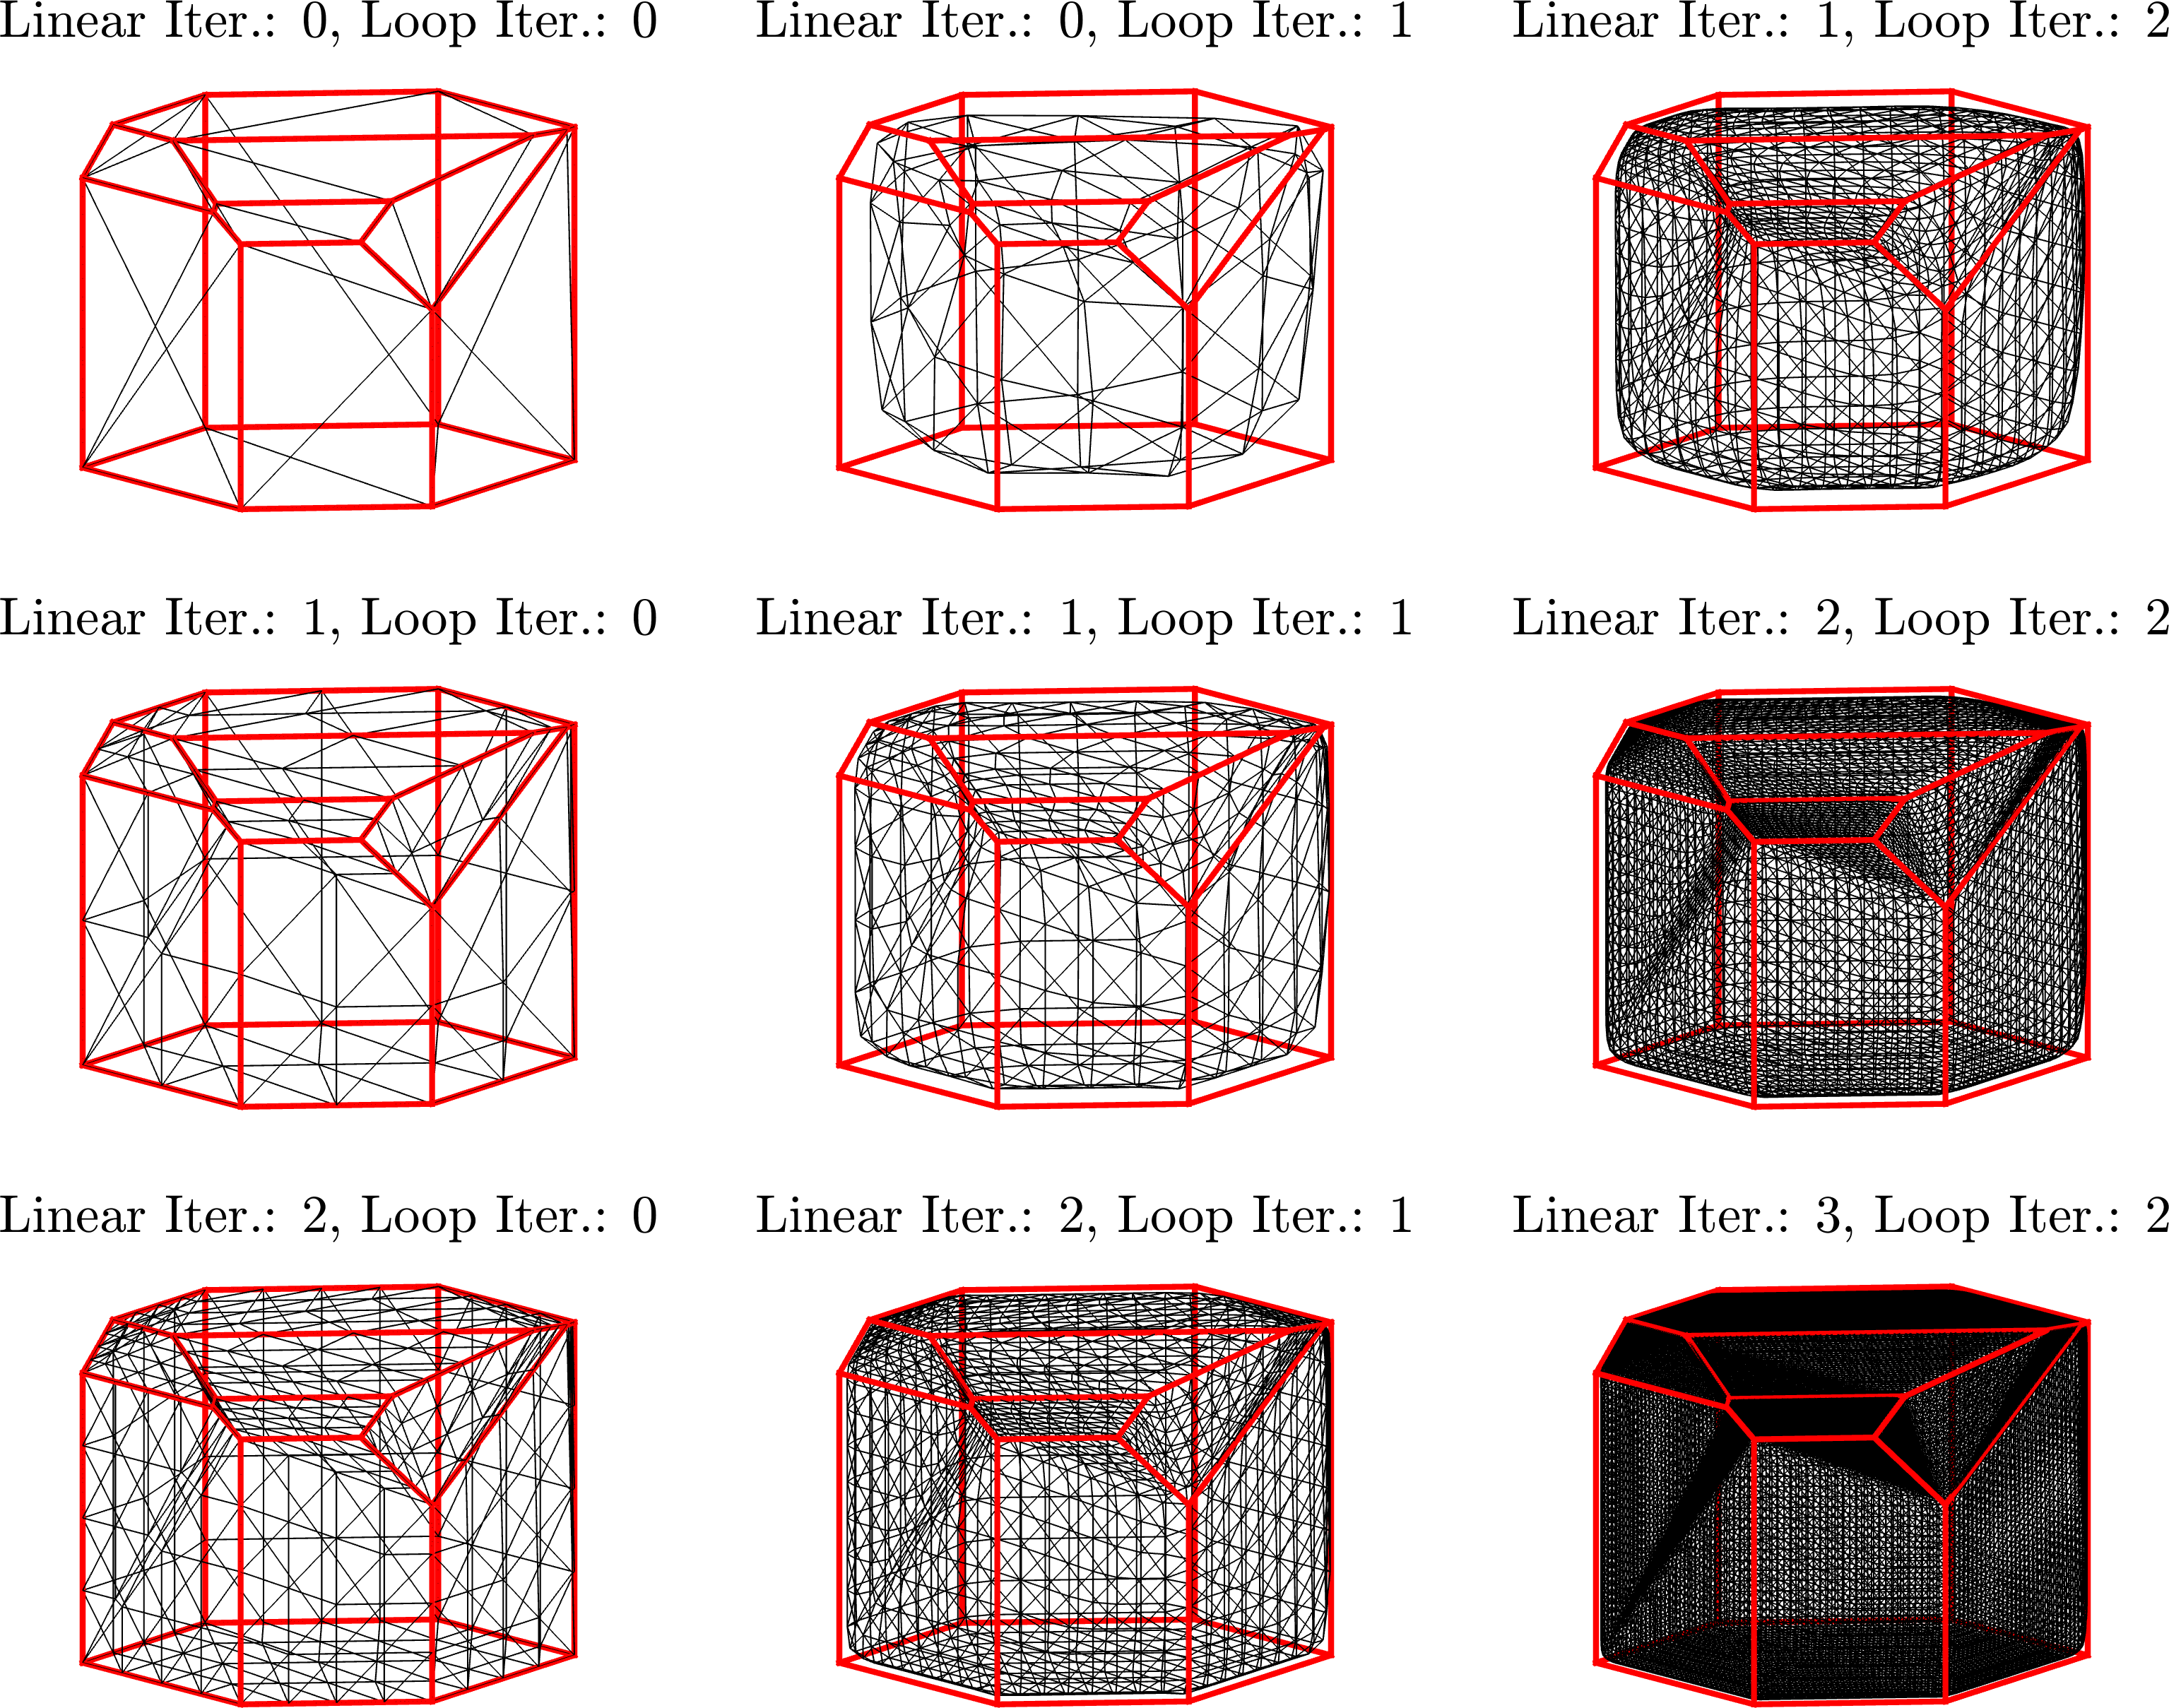
\includegraphics[width=350px]{subd_grid.png}
  \caption{Subdivided object (black) with reference (red) with various levels of subdivision}
  \label{fig:subd_grid}
\end{figure}

\subsubsection{Vertex Classification}

When introducing a concavity, it is important to classify which vertices are part of the concave feature --- and therefore need to be updated --- and which vertices should remain unaffected. This is accomplished by measuring the angle from each face normal to the EGI error vector, where faces with normal vectors within an angle of $\pi/2$ to the error vector must be updated. In reality, all face normals and areas are impacted by the presence of the concavity in the area optimization Eq. \ref{eq:area_opt_convex} and EGI correction step Eq \ref{eq:egi_validation}. Selecting the angle defect $\pi/2$ updates all faces above the horizon from the EGI error vector. This bound tends to produce visually accurate concavities. Faces requiring an update are termed \textit{free} faces, with all others termed \textit{root} faces.

Vertices on free faces are further classified as being \textit{root-adjacent} or \textit{free}. Root-adjacent vertices are part of at least one root face, whereas free vertices belong to only free faces. Classifying vertices in this way results in a border of root-adjacent vertices around the interior free vertices, visualized in Figure \ref{fig:root_and_free}.

\begin{figure}[!htb]
  \centering
  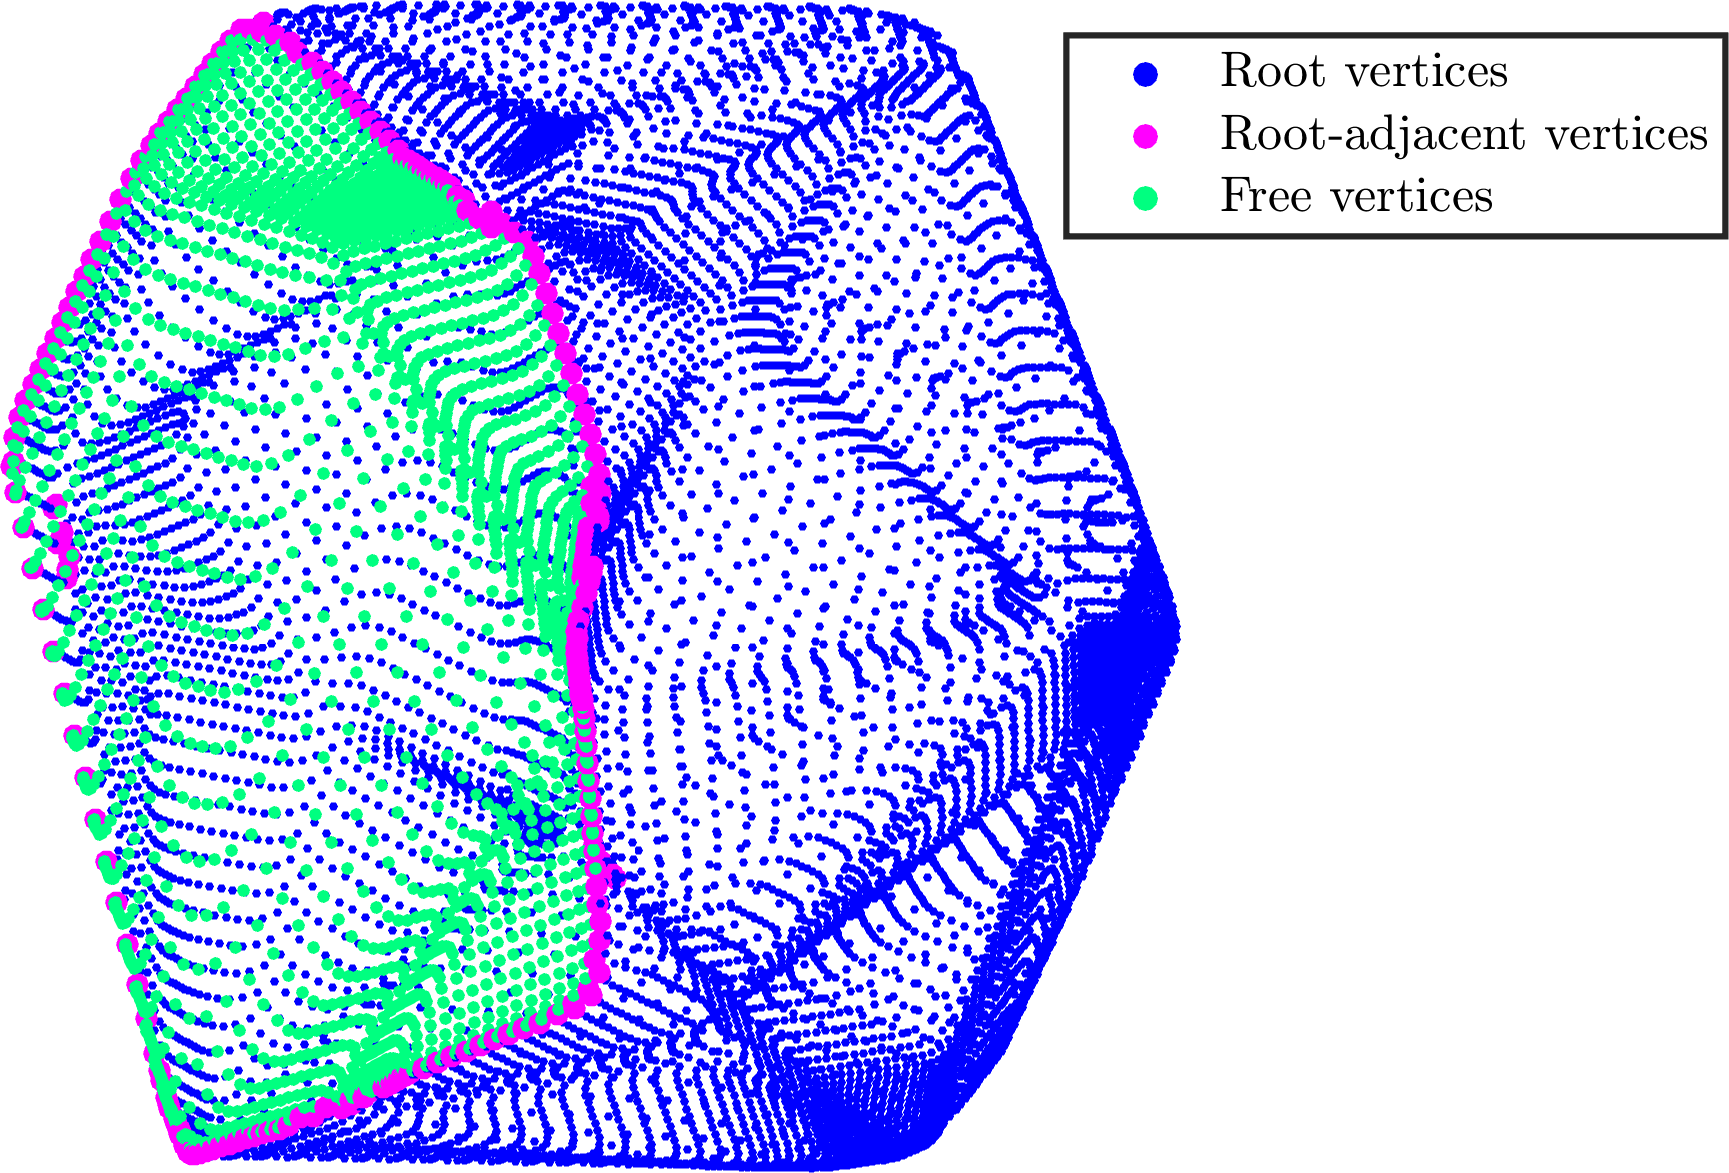
\includegraphics[width=250px]{rootadj_and_free_verts_try2.png}
  \caption{Root-adjacent and free vertices}
  \label{fig:root_and_free}
\end{figure}

\subsubsection{Vertex Displacement}

Given the estimated internal angle $\psi_{est}$ and the error vector $\hat{e}_{EGI}$, each $i$th free vertex is displaced to introduce a geometrically accurate concavity by moving each a distance $d_i$ in the direction of $-\hat{e}_{EGI}$:

\begin{equation} \label{eq:flip_depth}
  d_i = p_i \sqrt{\csc^2 \frac{\psi_{est}}{2} - 1},
\end{equation}

where $p_i$ is the distance from each $i$th free vertex to the nearest root-adjacent vertex.

\subsubsection{Internal Angle Iteration}

Prior work by the author indicated an analytical relationship between this interior angle and the norm of the EGI error vector, summarized in Figure \ref{fig:misleading_egi_error} \cite{robinson2022}.

\begin{figure}[!htb]
  \centering
  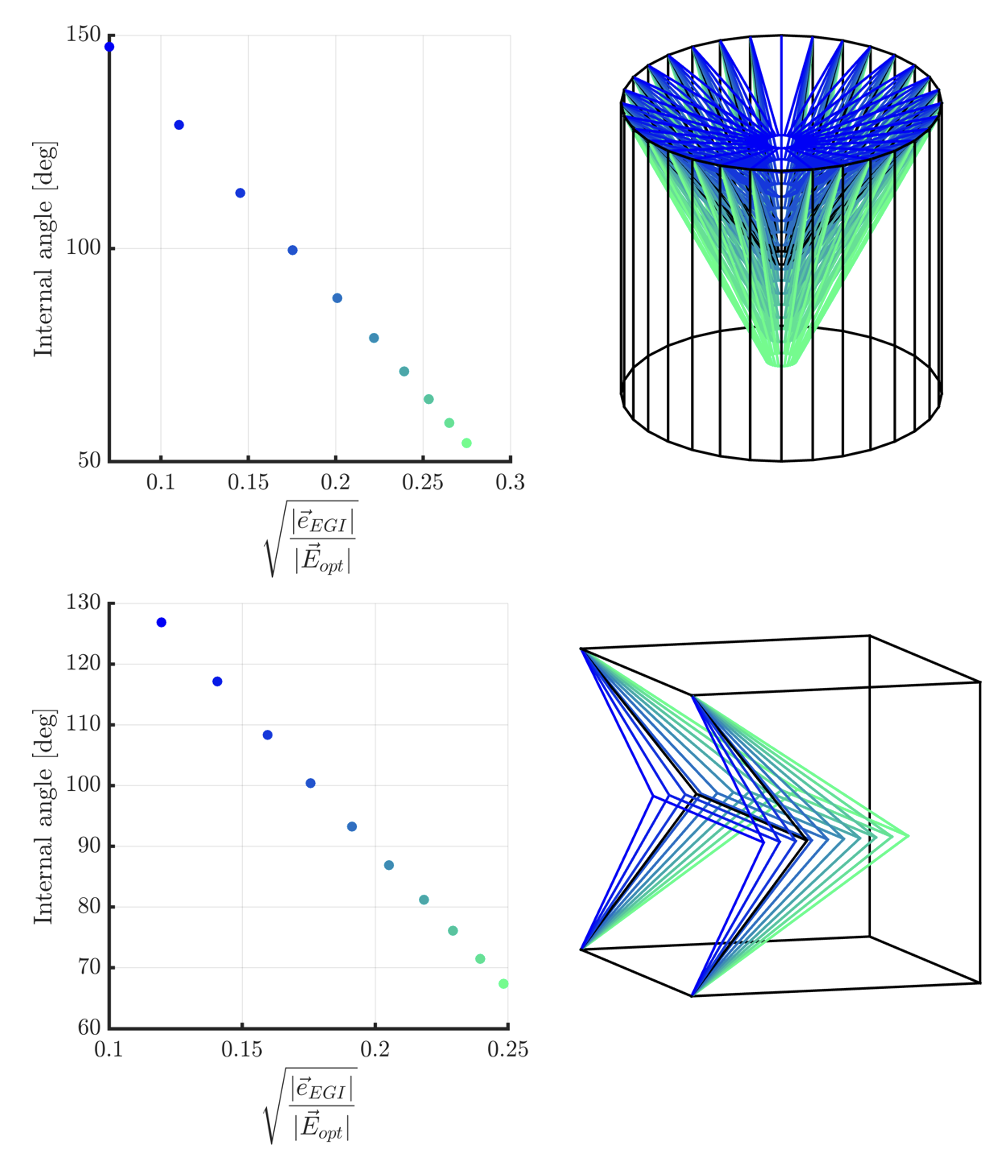
\includegraphics[width=\figsmall]{error_mag_study/combined_error_mag.png}
  \caption{EGI error relationship to internal angle for the collapsed cylinder and collapsed house from \cite{robinson2022}}
  \label{fig:misleading_egi_error}
\end{figure}

The objects in Figure \ref{fig:misleading_egi_error} were illuminated with a simple Lambertian BRDF and the brightness measurements used to optimize the EGI were produced by randomly sampled Sun and observer vectors. Once specular effects and non-random observation conditions are accounted for, the linear relationship between $\psi$ and $\sqrt{\frac{\|\vec{e}_{EGI}\|}{\|\vec{E}\|}}$ no longer exists. 

In practice, a line search is sufficient to find the interior angle that minimizes the light curve error of the reconstructed object, summarized in Algorithm \ref{alg:concavity_iter}.

\begin{algorithm}
  \caption{Concavity sizing algorithm}\label{alg:concavity_iter}
  \begin{algorithmic}
    \State $f_{cvx},v_{cvx}$ \Comment{Faces and vertices of the convex guess}
    \State $f_{subd}, \:v_{subd} \gets \mathrm{Subdivide}(f_{cvx},v_{cvx})$ \Comment{Subdivided convex guess}
    \State $\psi = 180^\circ$ \Comment{Initial guess, no concavity}
    \State $i = 0$ \Comment{Iteration number}
    \While {$i < i_{max}$}
      \State $f_{disp}, \:v_{disp} = \mathrm{DisplaceVertices}(f_{subd},v_{subd})$
      \State $\hat{I}_{i} = \mathrm{LightCurve}(f_{disp}, \:v_{disp})$
      \State $e_i = \| \hat{I} - \hat{I}_{i} \|$
      \State{$\psi \gets \psi + \Delta \psi$}
      \State{$i \gets i + 1$}
    \EndWhile

    $\psi_{opt} = \min_i{e_i}$
  \end{algorithmic}
\end{algorithm}

\subsection{Shape Inversion With Noisy Measurements}

\subsubsection{Shape Interpolation With Signed Distance Functions}

The signed distance field (SDF) implicitly represents a shape by associating each point in $\mathbb{R}^3$ with the distance to the closest point on the surface of the object \cite{baerentzen2002}. For a given SDF $f(x, y, z)$, the surface of the object is given by:

\begin{equation} \label{eq:sdf_zero_level_set}
  \begin{bmatrix} x \\ y \\ z \end{bmatrix} : \: \: f(x, y, z) = 0.
\end{equation}

Computing the SDF of a triangulated mesh breaks down into computing distances from the points, line segments, and planes making up the mesh to the queried point \cite{baerentzen2002}. A slice of the SDF of a test model is displayed in Figure \ref{fig:sdf_slice}.

\graphicspath{{/Users/liamrobinson/Documents/PyLightCurves/docs/build/html/_images}}
\begin{figure}[!htb]
  \centering
  \includegraphics[width=\figmed]{sphx_glr_sfds_001_2_00x.png}
  \caption{SDF slice of the Stanford bunny model}
  \label{fig:sdf_slice}
\end{figure}

Interpolating three-dimensional meshes using signed distance fields is not a novel concept of this work. Cohen-Or et al. used distance fields with anchor points to find warping functions between two geometries \cite{cohen_or1998}. A simpler, less robust interpolation strategy between two shapes can be accomplished through a weighted average of the respective SDFs. If both objects are weighted at $50\%$, the weighted sum of their SDFs produces a surface that lies halfway in between the two original shapes, measured perpendicular to the input objects' surfaces. This interpolated zero level set surface can be extracted through any three dimensional isocontouring algorithm such as marching cubes \cite{lorensen1987} or flying edges \cite{schroeder2015}. For example, interpolating between a torus and an icosahedron using this method yields Figure \ref{fig:interpolating_torus_ico}. 

\begin{figure}[!htb]
  \centering
  \includegraphics[width=\figmed]{sphx_glr_shape_interpolation_001.png}
  \caption{SDF interpolation between a torus and an icosahedron}
  \label{fig:interpolating_torus_ico}
\end{figure}

The proposed algorithm for shape interpolation for SDF interpolation of two shapes $M_1, M_2$ with convex weights $w_1, w_2$ is:

\begin{algorithm}
  \caption{SDF interpolation}\label{alg:sdf_interp}
  \begin{algorithmic}
  \Require $w_1 + w_2 = 1$
  \State $\mathrm{SDF}_{\textrm{interp}} \gets w_1 \cdot \mathrm{SDF}(M_1) + w_2 \cdot \mathrm{SDF}(M_2)$
  \State $M_{\textrm{interp}} = \mathrm{Isocontour}(\mathrm{SDF}_{\textrm{interp}}, 0)$.
  \end{algorithmic}
\end{algorithm}

Algorithm \ref{alg:sdf_interp} can operate on arbitrary convex or non-convex meshes, making it well suited to interpolating between light curve inversion results.

TODO: write

\chapter{Results}

\section{Realistic Light Curves}

\begin{figure}[!htb]
  \centering
  \includegraphics[width=\figbig]{sphx_glr_lc_uncertainty_002_2_00x.png}
  \caption{Light curves for a $1$-meter diffuse cube with $C_d = 0.5$ observed from the Purdue Optical Ground Station at \pogslla. Object is in the orbit of GOES 15 under torque-free rigid body motion with an inertia tensor $I = \mathrm{diag}(1.0, 2.0, 3.0) \: \left[kg \cdot m^2\right]$, $q_0 = \left[0, 0, 0, 1\right]^T$, $\omega_0 = \left[ 0.01, 0.02, 0.01 \right] \: \left[rad/s\right]$}
  \label{fig:cube_lcs}
\end{figure}

\clearpage
\section{Convex Shape Inversion Without Noise}

\subsection{Object Reconstruction Improvements}

The proposed resampling and merging steps in the object reconstruction process produce sparser results, in less computation time, with fewer convergence issues. Figure \ref{fig:egi_reconstructions} shows object reconstructions with each available EGI. The resampled EGIs does not converge in the maximum number of iterations evaluations ($100$) due to the density of faces with nearby normal vectors, causing large linearization errors the gradient estimation that lead to inefficient optimizer steps. It is clear that the final merged EGI produces the most accurate reconstruction of the truth object.

\begin{figure}[!htb]
  \centering
  \includegraphics[width=\figbig]{sphx_glr_aas_non_convex_inversion_002.png}
  \caption{Shape inversion results for convex objects without noise in the light curve}
  \label{fig:res_convex_no_noise}
\end{figure}

\clearpage
\section{Nonconvex Shape Inversion Without Noise}

Displacing free vertices in the EGI error vector direction by $d_i$ yields accurate concavities for objects whose concave boundaries lie in a plane. The result of applying this process to a set of representative convex objects is shown in Figure \ref{fig:res_convex_no_noise}.

The collapsed cube and icosahedron in Figure \ref{fig:res_convex_no_noise} are recovered effectively, but the collapsed house and box-wing satellite expose two limitations of the vertex displacement technique. In the case of the house where the concavity boundary is not constrained to a plane, the edges of the created concave feature are incorrect. The box-wing satellite's shadowing geometry leads the convex guess to be a poor approximation of the geometry outside of the concavity while also inheriting the same problem as the house.

This vertex displacement scheme will negligibly impact the convex guess if the truth object is also convex. A convex truth object will produce a small $\|\vec{e}_{EGI}\|$, causing the vertex update depth $d_{i}$ to trend towards zero as the estimated internal angle approaches $\psi = 180^\circ$. This is illustrated in Figure \ref{fig:non_convex_recon_of_convex} using the same input convex objects and attitude profiles as in Figure \ref{convex_grid}.


\begin{figure}[!htb]
  \centering
  \includegraphics[width=\figbig]{sphx_glr_aas_non_convex_inversion_003.png}
  \caption{Shape inversion results for nonconvex objects without noise in the light curve}
  \label{fig:res_nonconvex_no_noise}
\end{figure}

Figure \ref{fig:non_convex_recon_of_convex} clearly displays the compatibility of vertex displacement with truly convex objects. All objects are reconstructed faithfully in both their convex and nonconvex inversions, with the same caveats noted in the discussion following Figure \ref{convex_grid}. Some truly sharp edges are rounded during mesh subdivision as seen in the gem or rectangular prism. That said, others like the cylinder become more accurate as subdivision reintroduces continuity lost to discretization in EGI merging.

\clearpage
\section{Convex Shape Inversion With Noise}

\begin{figure}[!htb]
  \centering
  \includegraphics[width=\figbig]{sphx_glr_aas_non_convex_inversion_004.png}
  \caption{Shape inversion results for convex objects with noise in the light curve}
  \label{fig:res_convex_with_noise}
\end{figure}

TODO: this

\clearpage
\section{Nonconvex Shape Inversion With Noise}

\begin{figure}[!htb]
  \centering
  \includegraphics[width=\figbig]{sphx_glr_aas_non_convex_inversion_005.png}
  \caption{Shape inversion results for nonconvex objects with noise in the light curve}
  \label{fig:res_nonconvex_with_noise}
\end{figure}

TODO: this
